\documentclass{article}
\usepackage[dblblindworkshop]{neurips_2026}
\usepackage[utf8]{inputenc}
\usepackage[T1]{fontenc}
\usepackage{hyperref}
\usepackage{url}
\usepackage{booktabs}
\usepackage{amsfonts}
\usepackage{amsmath}
\usepackage{nicefrac}
\usepackage{microtype}
\usepackage{xcolor}
\usepackage{graphicx}
\usepackage{multirow}
\usepackage{caption}
\usepackage{float}
\captionsetup{font=small}

\workshoptitle{Machine Learning for Spatially Resolved High-dimensional Biology (ml4spatialbio)}

\title{Does spatial context transfer? Neighbourhood-aware cell typing in seminiferous tubules under tissue-organization and species shift}

\author{%
  Anonymous Author(s)\\
  Affiliation\\
  \texttt{email}
}

\begin{document}

\maketitle

\begin{abstract}
Methods for annotating spatial transcriptomics data increasingly use a spot's tissue neighbourhood as input, but they are benchmarked within one tissue and condition, so it is unknown whether the spatial signal they learn holds when tissue organization changes. We build a small benchmark from the public Slide-seqV2 testis pucks of Chen et al.\ (2021): three wild-type mouse, three diabetic \emph{ob/ob} mouse, and two human pucks (252,898 beads), with cell-type labels from NMFreg (non-negative matrix factorization regression). Using germ-cell stage annotation in seminiferous tubules as the task, we compare an expression-only classifier with neighbourhood-augmented features, a GraphSAGE model, and test-time smoothing of the expression-only posterior, under held-out-puck, wild-type-to-\emph{ob/ob}, and mouse-to-human transfer. Spatial context adds about one macro-F1 point within a species and up to three on human pucks. The \emph{ob/ob} pucks are not a distribution shift for this task. Across species, expression-only accuracy drops by ten points; neighbourhood-augmented features and test-time smoothing keep their gains, whereas GraphSAGE, which matches them within a species, becomes the worst model, losing five points and fifteen F1 points on round spermatids. The gain from context tracks how informative the neighbourhood is relative to the bead itself rather than the target tissue's neighbourhood homogeneity. Fixed spatial aggregation transfers across the shifts we tested where learned spatial features do not.

\end{abstract}

\section{Introduction}
Most recent methods for annotating cells or beads in spatial transcriptomics use the tissue neighbourhood of a spot as an additional input, either by concatenating a spot's own expression with an aggregate of its neighbours' \citep{singhal2024banksy, varrone2024cellcharter} or by learning a graph neural network over a spatial adjacency graph \citep{hu2021spagcn, dong2022deciphering, long2023spatially}. Benchmarks of these methods \citep{yuan2024benchmarking, li2022benchmarking} evaluate within one tissue and one condition, so they do not tell us whether the spatial signal a model learns still holds when tissue organization changes, which is the question that matters when a model trained on a reference is used to annotate samples from other conditions, individuals, or species.

The testis is a natural place to ask it. Spermatogenesis proceeds inside seminiferous tubules along a radial axis, from spermatogonia at the basement membrane through spermatocytes and round spermatids to elongating spermatids at the lumen, and tubule cross-sections cycle through a fixed sequence of stages \citep{hess2008spermatogenesis, chakravorty2026temporal}. The same layering exists in mouse and human, but the human cycle differs in stage number and in how stages tile a cross-section. \citet{chen2021dissecting} produced Slide-seqV2 \citep{stickels2021highly} pucks of wild-type mouse testis, of testis from diabetic \emph{ob/ob} mice, in which they report disrupted spatial organization of the tubules, and of normal human testis, each with bead-level cell-type labels from NMFreg \citep{rodriques2019slide}. This gives three levels of distribution shift on one tissue with one platform and one labelling procedure: a held-out puck of the same condition, a condition that alters tissue organization, and a different species.

We ask how much spatial context improves bead-level annotation of germ-cell stage, and whether the improvement survives each shift, comparing an expression-only classifier against neighbourhood-augmented features, a graph neural network, and test-time smoothing of the expression-only posterior over the target puck's spatial graph. The last is trained without any spatial input and uses the target tissue's geometry only at inference, separating the value of a spatial prior from the transferability of learned spatial features.


\section{Data and task}
\paragraph{Pucks.} We use the eight processed Slide-seqV2 pucks released by \citet{chen2021dissecting}: three wild-type (WT) mouse, three \emph{ob/ob} diabetic (DB) mouse, and two normal human (HU) pucks, each with a bead-by-gene count matrix, bead coordinates, and a per-bead NMFreg label over nine types (spermatogonia SPG, spermatocytes SPC, round spermatids RS, elongating/elongated spermatids ES, Sertoli, myoid, Leydig, endothelial, macrophage). We keep beads with a label and at least 100 UMIs, leaving 25,377 to 39,181 beads per puck (252,898 in total; Table~\ref{tab:homog}).

\paragraph{Cross-species gene space.} All pucks are restricted to one-to-one mouse--human orthologs from MGI \citep{baldarelli2024mouse} detected in every puck (13,573 genes), so a model trained on mouse can be applied to human without adaptation. Counts are library-size normalized and log-transformed \citep{wolf2018scanpy}. We select 2,000 highly variable genes on the WT pucks only \citep{stuart2019comprehensive}, then standardize each gene within each puck using that puck's own mean and standard deviation. This unsupervised per-puck standardization is the only batch handling we apply.

\paragraph{Task.} The primary task is four-class germ-cell stage annotation (SPG, SPC, RS, ES) on germ-cell beads, which are 81 to 90\% of beads. This is the layer the radial tubule axis defines, and the reproducible part of the NMFreg annotation: within-puck and cross-puck macro-F1 agree (0.71 vs.\ 0.70), whereas the rare somatic types (endothelial, macrophage, myoid) are near chance from a single bead's expression under any split. Six-class and nine-class variants are in the appendix.

\paragraph{Shift settings.} Training pucks are always disjoint from the test puck. \emph{WT$\to$WT}: train on two WT pucks, test on the third (three folds). \emph{WT$\to$ob/ob}: train on all three WT pucks, test on each DB puck. \emph{WT$\to$human}: train on all three WT pucks, test on each human puck; \emph{mouse$\to$human} adds the DB pucks to training. As in-distribution references for the shifted targets, \emph{ob/ob$\to$ob/ob} and \emph{human$\to$human} train on the other pucks of the same condition. The NMFreg labels were computed from expression alone, so a gain from spatial features cannot be an artefact of how the labels were made. For each puck we also compute neighbourhood homogeneity, the mean fraction of a bead's 15 nearest spatial neighbours that share its label; it is used only to describe the pucks, never as an input. Among germ-cell beads it is 0.53 to 0.56 on WT, 0.49 to 0.57 on \emph{ob/ob}, and 0.38 to 0.40 on human pucks.


\section{Models and evaluation protocol}
All models operate on a 50-dimensional PCA embedding $z_i$ of the standardized expression, with the PCA fit on the training pucks only and applied to the test puck. Let $\mathcal{N}_k(i)$ be the $k$ nearest spatial neighbours of bead $i$ within its puck, and $\bar z_i^{(k)} = \frac{1}{k}\sum_{j\in\mathcal{N}_k(i)} z_j$ the neighbourhood mean. Neighbourhoods are computed over all beads of a puck, including non-germ beads, since context is label-free.

\paragraph{Expression only.} A multinomial logistic regression (LR) on $z_i$, and a two-layer MLP (256 hidden units, dropout 0.2). Both use class-balanced loss weights.

\paragraph{Neighbourhood-augmented features.} LR and MLP on $[z_i, \bar z_i^{(k)}]$, the construction used by BANKSY \citep{singhal2024banksy} and related methods, for $k\in\{5,15,30\}$. As a diagnostic we also fit LR on $\bar z_i^{(k)}$ alone, i.e.\ on the surroundings without the bead.

\paragraph{Graph neural network.} A two-layer GraphSAGE with mean aggregation \citep{hamilton2017inductive}, $h_i' = \sigma(W_1 h_i + W_2 \bar h_i^{(15)})$, 128 hidden units, trained full-batch on the union of training pucks (each puck is its own connected graph) and applied to the test puck's graph.

\paragraph{Test-time smoothing.} We take the expression-only LR posterior $p_i$ on the test puck and replace it with $p_i' = (1-\alpha)\,p_i + \alpha\,\bar p_i^{(15)}$, then predict $\arg\max p_i'$. This is one step of label propagation on the model's own outputs \citep{huang2021combining}; it uses the target puck's geometry but no spatial input during training, so any gain reflects the target tissue's local homogeneity rather than transferred spatial features. We sweep $\alpha\in\{0.25,0.5,0.75,1\}$.

\paragraph{Evaluation.} Macro-F1 over the classes present in the test puck and per-class F1, averaged over seeds (three for MLP and GraphSAGE; LR is deterministic) and then over the test pucks of a setting, with the standard deviation across test pucks. The full grid runs on two CPU cores in a few hours.


\section{Results}
\begin{table}[t]
\centering
\caption{Macro-F1 for germ-cell stage annotation under six train/test settings (left three in-distribution, right three shifted); mean over test pucks, $\pm$ standard deviation across test pucks. nbr: mean embedding of the 15 nearest spatial neighbours. $\alpha$ was selected on the WT$\to$WT folds. MLP rows are in Table~\ref{tab:germ4full}.}
\label{tab:main}
\footnotesize
\setlength{\tabcolsep}{2.5pt}
\input{../results/table_germ4_main.tex}
\end{table}

\begin{figure}[t]
\centering
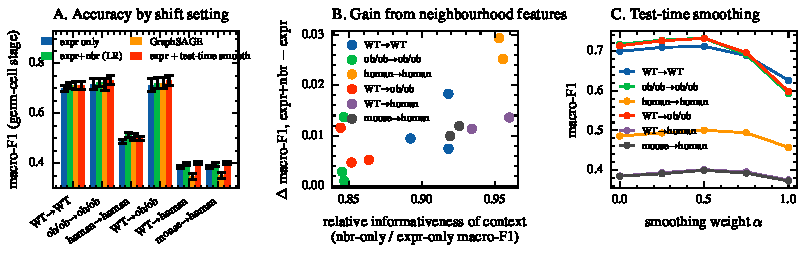
\includegraphics[width=\linewidth]{figs/fig_main.pdf}
\caption{(A) Germ-cell stage macro-F1 by shift setting; error bars are standard deviations across test pucks. (B) Gain from neighbourhood features per test puck against the relative informativeness of context (macro-F1 of a neighbourhood-only classifier divided by that of the expression-only classifier). (C) Test-time smoothing of the expression-only posterior against the weight $\alpha$; $\alpha=1$ replaces each bead's posterior by its neighbours' mean.}
\label{fig:main}
\end{figure}

\paragraph{In-distribution gains are small and consistent.} On held-out WT pucks, the expression-only logistic regression reaches 0.699 macro-F1, and every form of spatial context adds about one point: neighbourhood-augmented LR 0.711, GraphSAGE 0.711, and test-time smoothing 0.712 (Table~\ref{tab:main}, Fig.~\ref{fig:main}A). The neighbourhood alone, without the bead's own expression, reaches 0.636, so most of the stage signal is in the bead itself. Gains are similar on \emph{ob/ob} and larger on human folds, where the expression-only ceiling is lower (0.486) and neighbourhood features add 2.7 points (0.513). Neighbourhood size matters little: $k\in\{5,15,30\}$ changes macro-F1 by at most 0.008 (Table~\ref{tab:sweeps}). An MLP on the same features is 0.6 to 2.1 points below the LR in every setting (Table~\ref{tab:germ4full}).

\paragraph{The \emph{ob/ob} shift is small for this task.} Models trained on WT pucks and applied to \emph{ob/ob} pucks perform as well as models trained on other \emph{ob/ob} pucks (0.713 vs.\ 0.717 for expression only; 0.721 vs.\ 0.723 with neighbourhood features). The spatial gains carry over unchanged, and germ-cell homogeneity overlaps between conditions (0.49 to 0.57 vs.\ 0.53 to 0.56), so at this resolution the disruption reported by \citet{chen2021dissecting} does not register as a distribution shift for stage annotation.

\paragraph{Species shift is large and is dominated by expression.} Expression-only macro-F1 falls from 0.486 (human$\to$human) to 0.385 (WT$\to$human), and adding the \emph{ob/ob} pucks to training does not change it (0.385). Neighbourhood-augmented LR retains a gain under species shift (0.398, $+1.3$), as does test-time smoothing (0.401, $+1.6$). GraphSAGE does not: it is within 0.008 of neighbourhood-augmented LR in every in-distribution setting and becomes the worst model across species, at 0.347 ($-3.8$ vs.\ expression only, $-5.1$ vs.\ neighbourhood LR; seed-to-seed SD $\le 0.007$). Per stage (Fig.~\ref{fig:perclass} in the appendix), the loss is concentrated on round spermatids, the largest human class, whose F1 drops from 0.390 to 0.237 with GraphSAGE and to 0.376 with neighbourhood LR; with neighbourhood LR, spermatogonia and spermatocytes still gain about 3 points.

\paragraph{What predicts the gain.} The gain from context does not track the neighbourhood homogeneity of the target puck: the largest gains occur on the human pucks, which have the lowest homogeneity (0.38 to 0.40). What tracks the gain is instead how informative the neighbourhood is relative to the bead (Fig.~\ref{fig:main}B): the ratio of neighbourhood-only to expression-only macro-F1 is 0.84 to 0.92 for mouse targets, where gains are 0.1 to 1.8 points, and 0.92 to 0.96 for human targets, where gains are 1.0 to 2.9 points. Test-time smoothing peaks at $\alpha=0.5$ in every setting (Fig.~\ref{fig:main}C); replacing the bead's posterior by its neighbours' ($\alpha=1$) costs 7 to 12 points on mouse and 1 to 3 on human targets. At the bead level, the within-species gain is concentrated in the lowest-UMI tertile ($+2.3$ accuracy points on WT$\to$WT, $+4.7$ on human$\to$human, near zero elsewhere), and context lowers accuracy for beads whose neighbourhoods are heterogeneous (Table~\ref{tab:strat}).



\section{Discussion}
On this benchmark, spatial context is worth about one macro-F1 point for germ-cell stage annotation within a species and up to three points on human pucks, where the bead's own expression is a weaker signal. The value is small because the neighbourhood is mostly redundant with the bead: a bead's stage is predictable from its 15 neighbours alone at 0.61 to 0.64 macro-F1 in mouse, but this is largely the information the bead already carries. We would not expect this to hold for niche-level labels, where the neighbourhood defines the class. Two further negative results follow. The \emph{ob/ob} pucks, which \citet{chen2021dissecting} used to show disrupted tubule organization, are not a distribution shift for stage annotation, so organization changes that matter for niche-level analysis can be invisible at this level. And neighbourhood homogeneity of the target tissue does not predict how much context helps; the relative informativeness of the neighbourhood does, but it requires target labels and is therefore a diagnostic rather than a predictor.

The more useful result is the split between how context is used. Fixed aggregation followed by a linear model, and post-hoc smoothing of a spatial-free model, keep their gains under both shifts we tested. A two-layer GNN matches them within a species and loses about five points relative to them across species. The GNN's first layer sees exactly the neighbourhood mean the linear model sees; its later layers learn a nonlinear function of the mouse neighbourhood distribution that does not hold for human tubules, with the loss falling almost entirely on round spermatids. \citet{huang2021combining} reached a related conclusion for citation graphs, that simple models plus label propagation match GNNs; here the argument is about robustness rather than accuracy. For reference-based annotation across species, which is how spatial atlases will most often be applied, a model whose spatial component is a fixed operator has an advantage that in-distribution benchmarks do not reveal.

\paragraph{Limitations.} Labels are NMFreg assignments rather than ground truth, and the human labels are noisier than the mouse ones (in-distribution ceiling 0.49 vs.\ 0.70), so results are agreement with a published annotation; the human estimates rest on two pucks. The cross-species gene space is one-to-one orthologs with mouse-selected variable genes, and the only batch handling is per-puck standardization; stronger integration \citep{rosen2024toward, lotfollahi2022mapping} would likely narrow the species gap for all models, and whether it would close the GNN's gap is open. We evaluated one GNN at one depth. Code and splits will be released.


\bibliographystyle{plainnat}
\bibliography{refs}

\clearpage
\appendix
\section{Additional results}
\begin{table}[H]
\centering
\caption{Puck statistics after filtering. Homogeneity is the mean fraction of a bead's $k$ nearest spatial neighbours that share its NMFreg label, over all beads (k=5, 15, 30) and over germ-cell beads only (k=15).}
\label{tab:homog}
\small
\begin{tabular}{lrrrrrrr}
\toprule
Puck & Condition & Beads & Median UMI & Homog. $k$=5 & $k$=15 & $k$=30 & Germ, $k$=15 \\
\midrule
WT1 & WT mouse & 29,178 & 719 & 0.524 & 0.474 & 0.432 & 0.538 \\
WT2 & WT mouse & 29,607 & 782 & 0.524 & 0.470 & 0.426 & 0.533 \\
WT3 & WT mouse & 39,181 & 604 & 0.561 & 0.507 & 0.464 & 0.561 \\
DB1 & \emph{ob/ob} mouse & 25,377 & 797 & 0.484 & 0.426 & 0.385 & 0.485 \\
DB2 & \emph{ob/ob} mouse & 35,629 & 426 & 0.537 & 0.477 & 0.433 & 0.530 \\
DB3 & \emph{ob/ob} mouse & 30,073 & 684 & 0.574 & 0.518 & 0.473 & 0.568 \\
HU1 & human & 30,464 & 602 & 0.362 & 0.336 & 0.316 & 0.380 \\
HU2 & human & 33,389 & 600 & 0.379 & 0.352 & 0.331 & 0.397 \\
\bottomrule
\end{tabular}
\end{table}

\begin{figure}[H]
\centering
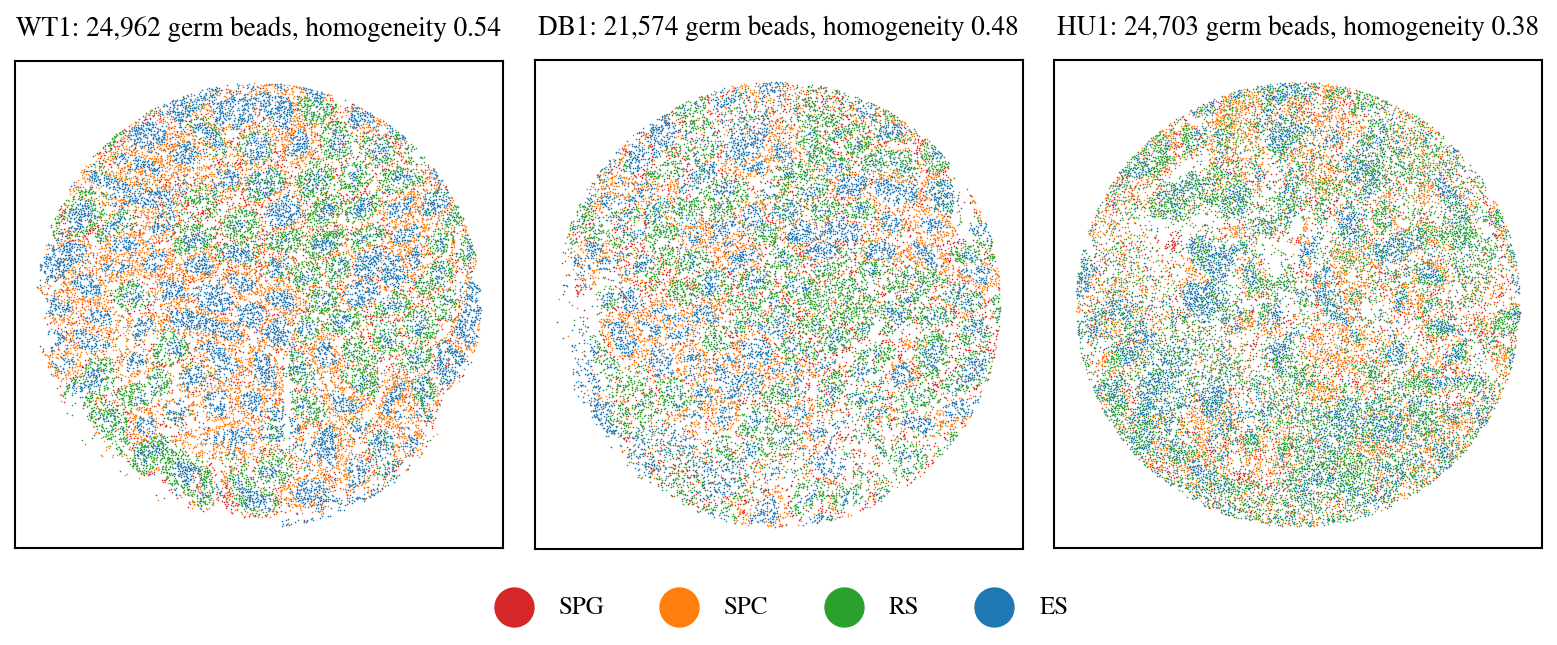
\includegraphics[width=0.95\linewidth]{figs/fig_pucks.png}
\caption{Germ-cell beads of one WT mouse, one \emph{ob/ob} mouse, and one human puck, coloured by NMFreg stage. Tubule cross-sections with a spermatogonia/spermatocyte rim and a spermatid core are visible in mouse; human tubules are larger and stage labels are more mixed.}
\label{fig:pucks}
\end{figure}

\begin{table}[H]
\centering
\caption{Full version of Table~\ref{tab:main}, including the MLP models. Macro-F1, mean $\pm$ SD across test pucks.}
\label{tab:germ4full}
\footnotesize
\setlength{\tabcolsep}{2.5pt}
\begin{tabular}{lcccccc}
\toprule
Model & WT→WT & ob/ob→ob/ob & human→human & WT→ob/ob & WT→human & mouse→human \\
\midrule
LR (expr) & 0.699\,{\scriptsize$\pm$0.013} & 0.717\,{\scriptsize$\pm$0.022} & 0.486\,{\scriptsize$\pm$0.008} & 0.713\,{\scriptsize$\pm$0.026} & 0.385\,{\scriptsize$\pm$0.005} & 0.385\,{\scriptsize$\pm$0.006} \\
LR (expr+nbr) & 0.711\,{\scriptsize$\pm$0.013} & 0.723\,{\scriptsize$\pm$0.016} & 0.513\,{\scriptsize$\pm$0.011} & 0.721\,{\scriptsize$\pm$0.023} & 0.398\,{\scriptsize$\pm$0.007} & 0.396\,{\scriptsize$\pm$0.008} \\
LR (nbr only) & 0.636\,{\scriptsize$\pm$0.003} & 0.607\,{\scriptsize$\pm$0.019} & 0.464\,{\scriptsize$\pm$0.006} & 0.609\,{\scriptsize$\pm$0.029} & 0.365\,{\scriptsize$\pm$0.012} & 0.355\,{\scriptsize$\pm$0.008} \\
LR (expr) + smooth ($\alpha$=0.5) & 0.712\,{\scriptsize$\pm$0.016} & 0.733\,{\scriptsize$\pm$0.019} & 0.501\,{\scriptsize$\pm$0.008} & 0.732\,{\scriptsize$\pm$0.021} & 0.401\,{\scriptsize$\pm$0.005} & 0.400\,{\scriptsize$\pm$0.006} \\
MLP (expr) & 0.693\,{\scriptsize$\pm$0.014} & 0.704\,{\scriptsize$\pm$0.036} & 0.475\,{\scriptsize$\pm$0.012} & 0.704\,{\scriptsize$\pm$0.028} & 0.370\,{\scriptsize$\pm$0.009} & 0.369\,{\scriptsize$\pm$0.009} \\
MLP (expr+nbr) & 0.705\,{\scriptsize$\pm$0.018} & 0.708\,{\scriptsize$\pm$0.029} & 0.498\,{\scriptsize$\pm$0.014} & 0.713\,{\scriptsize$\pm$0.023} & 0.378\,{\scriptsize$\pm$0.013} & 0.375\,{\scriptsize$\pm$0.011} \\
GraphSAGE & 0.711\,{\scriptsize$\pm$0.015} & 0.716\,{\scriptsize$\pm$0.023} & 0.505\,{\scriptsize$\pm$0.013} & 0.721\,{\scriptsize$\pm$0.023} & 0.347\,{\scriptsize$\pm$0.012} & 0.350\,{\scriptsize$\pm$0.012} \\
\bottomrule
\end{tabular}

\end{table}

\begin{figure}[H]
\centering
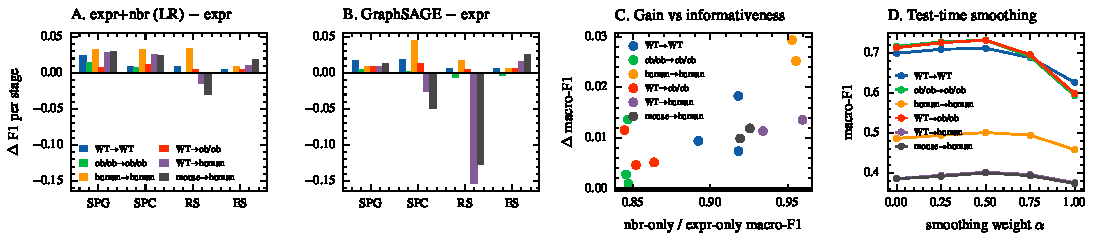
\includegraphics[width=0.8\linewidth]{figs/fig_perclass.pdf}
\caption{(A, B) Per-stage change in F1 from adding spatial context, relative to the expression-only LR, in all six settings; shared vertical scale. (C) Gain from neighbourhood features per test puck against the relative informativeness of context. (D) Test-time smoothing of the expression-only posterior against the weight $\alpha$; $\alpha=1$ replaces each bead's posterior by its neighbours' mean.}
\label{fig:perclass}
\end{figure}

\paragraph{Neighbourhood size and smoothing weight.} Table~\ref{tab:sweeps} reports the LR with neighbourhood features for $k\in\{5,15,30\}$ and test-time smoothing for all $\alpha$.

\begin{table}[H]
\centering
\caption{Sensitivity to neighbourhood size $k$ (LR on expression plus neighbourhood mean) and to the smoothing weight $\alpha$ (expression-only LR posterior smoothed over the test puck's 15-NN graph). Macro-F1 for germ-cell stage, mean over test pucks.}
\label{tab:sweeps}
\small
\begin{tabular}{lccc|ccccc}
\toprule
 & \multicolumn{3}{c|}{expr+nbr, $k$} & \multicolumn{5}{c}{smoothing weight $\alpha$} \\
Setting & 5 & 15 & 30 & 0 & 0.25 & 0.5 & 0.75 & 1 \\
\midrule
WT→WT & 0.715 & 0.711 & 0.708 & 0.699 & 0.709 & 0.712 & 0.689 & 0.626 \\
ob/ob→ob/ob & 0.728 & 0.723 & 0.720 & 0.717 & 0.728 & 0.733 & 0.691 & 0.593 \\
human→human & 0.511 & 0.513 & 0.510 & 0.486 & 0.494 & 0.501 & 0.494 & 0.457 \\
WT→ob/ob & 0.722 & 0.721 & 0.718 & 0.713 & 0.726 & 0.732 & 0.696 & 0.598 \\
WT→human & 0.399 & 0.398 & 0.394 & 0.385 & 0.393 & 0.401 & 0.395 & 0.375 \\
mouse→human & 0.397 & 0.396 & 0.390 & 0.385 & 0.391 & 0.400 & 0.392 & 0.373 \\
\bottomrule
\end{tabular}

\end{table}

\paragraph{Six-class and nine-class labels.} Tables~\ref{tab:coarse6} and \ref{tab:full9} repeat the linear models on all beads with a six-class scheme (four germ stages, tubular somatic, interstitial) and with the original nine NMFreg labels. Macro-F1 is much lower for nine classes because the rare somatic types (endothelial, macrophage, myoid) are near chance from a single bead's expression even in-distribution. The gains from context are smaller than for germ-cell stage (0.4 to 1.0 points within a species for six classes, none for nine classes) but again largest on human in-distribution folds (about two points); across species with nine classes, neither neighbourhood features nor smoothing changes macro-F1 by more than 0.004.

\begin{table}[H]
\centering
\caption{Six-class annotation (SPG, SPC, RS, ES, tubular somatic, interstitial), all beads. Macro-F1, mean $\pm$ SD across test pucks.}
\label{tab:coarse6}
\footnotesize
\setlength{\tabcolsep}{2.5pt}
\begin{tabular}{lcccccc}
\toprule
Model & WT→WT & ob/ob→ob/ob & human→human & WT→ob/ob & WT→human & mouse→human \\
\midrule
LR (expr) & 0.524\,{\scriptsize$\pm$0.018} & 0.549\,{\scriptsize$\pm$0.010} & 0.418\,{\scriptsize$\pm$0.001} & 0.547\,{\scriptsize$\pm$0.009} & 0.301\,{\scriptsize$\pm$0.004} & 0.299\,{\scriptsize$\pm$0.006} \\
LR (expr+nbr) & 0.533\,{\scriptsize$\pm$0.017} & 0.553\,{\scriptsize$\pm$0.007} & 0.441\,{\scriptsize$\pm$0.002} & 0.553\,{\scriptsize$\pm$0.007} & 0.308\,{\scriptsize$\pm$0.003} & 0.306\,{\scriptsize$\pm$0.002} \\
LR (nbr only) & 0.453\,{\scriptsize$\pm$0.003} & 0.429\,{\scriptsize$\pm$0.013} & 0.391\,{\scriptsize$\pm$0.006} & 0.435\,{\scriptsize$\pm$0.017} & 0.280\,{\scriptsize$\pm$0.007} & 0.278\,{\scriptsize$\pm$0.007} \\
LR (expr) + smooth ($\alpha$=0.5) & 0.531\,{\scriptsize$\pm$0.018} & 0.558\,{\scriptsize$\pm$0.016} & 0.433\,{\scriptsize$\pm$0.000} & 0.561\,{\scriptsize$\pm$0.012} & 0.316\,{\scriptsize$\pm$0.006} & 0.315\,{\scriptsize$\pm$0.002} \\
\bottomrule
\end{tabular}

\end{table}

\begin{table}[H]
\centering
\caption{Nine-class annotation with the original NMFreg labels, all beads. Macro-F1, mean $\pm$ SD across test pucks.}
\label{tab:full9}
\footnotesize
\setlength{\tabcolsep}{2.5pt}
\begin{tabular}{lcccccc}
\toprule
Model & WT→WT & ob/ob→ob/ob & human→human & WT→ob/ob & WT→human & mouse→human \\
\midrule
LR (expr) & 0.390\,{\scriptsize$\pm$0.005} & 0.405\,{\scriptsize$\pm$0.000} & 0.309\,{\scriptsize$\pm$0.002} & 0.409\,{\scriptsize$\pm$0.010} & 0.181\,{\scriptsize$\pm$0.006} & 0.182\,{\scriptsize$\pm$0.003} \\
LR (expr+nbr) & 0.392\,{\scriptsize$\pm$0.004} & 0.401\,{\scriptsize$\pm$0.004} & 0.330\,{\scriptsize$\pm$0.001} & 0.413\,{\scriptsize$\pm$0.012} & 0.177\,{\scriptsize$\pm$0.005} & 0.180\,{\scriptsize$\pm$0.004} \\
LR (nbr only) & 0.316\,{\scriptsize$\pm$0.004} & 0.296\,{\scriptsize$\pm$0.010} & 0.280\,{\scriptsize$\pm$0.005} & 0.305\,{\scriptsize$\pm$0.007} & 0.160\,{\scriptsize$\pm$0.006} & 0.168\,{\scriptsize$\pm$0.002} \\
LR (expr) + smooth ($\alpha$=0.5) & 0.393\,{\scriptsize$\pm$0.006} & 0.412\,{\scriptsize$\pm$0.010} & 0.328\,{\scriptsize$\pm$0.001} & 0.416\,{\scriptsize$\pm$0.014} & 0.179\,{\scriptsize$\pm$0.005} & 0.181\,{\scriptsize$\pm$0.003} \\
\bottomrule
\end{tabular}

\end{table}

\paragraph{Gain by sequencing depth and local homogeneity.} Table~\ref{tab:strat} stratifies the accuracy gain from neighbourhood features by the test bead's UMI tertile and by the fraction of its 15 neighbours that share its label. Within a species the gain comes from low-UMI beads; under species shift it comes from high-UMI beads. In every setting context lowers accuracy for beads with heterogeneous neighbourhoods (fewer than 40\% same-label neighbours) and raises it for the rest, so the puck-level gain is a net of these two effects.

\begin{table}[H]
\centering
\caption{Accuracy gain from neighbourhood features (expr+nbr minus expr, LR) stratified by the test bead's UMI tertile within its puck and by its local label homogeneity. Mean over test pucks of each setting.}
\label{tab:strat}
\small
\begin{tabular}{lccc|ccccc}
\toprule
 & \multicolumn{3}{c|}{UMI tertile} & \multicolumn{5}{c}{local homogeneity} \\
Setting & low & mid & high & 0-0.2 & 0.2-0.4 & 0.4-0.6 & 0.6-0.8 & 0.8-1 \\
\midrule
WT→WT & +0.023 & +0.003 & +0.003 & -0.023 & -0.010 & +0.022 & +0.030 & +0.018 \\
ob/ob→ob/ob & +0.015 & -0.001 & -0.002 & -0.036 & -0.011 & +0.017 & +0.024 & +0.019 \\
human→human & +0.047 & +0.021 & +0.018 & -0.048 & +0.014 & +0.091 & +0.111 & +0.089 \\
WT→ob/ob & +0.015 & +0.002 & +0.003 & -0.035 & -0.009 & +0.019 & +0.030 & +0.021 \\
WT→human & -0.011 & +0.002 & +0.029 & +0.000 & -0.007 & +0.011 & +0.034 & +0.050 \\
mouse→human & -0.001 & +0.004 & +0.016 & -0.007 & -0.001 & +0.013 & +0.033 & +0.042 \\
\bottomrule
\end{tabular}

\end{table}

\paragraph{Representation shift.} Table~\ref{tab:shift} reports both measures of how far the feature distribution moves between training and test pucks: the AUC of a logistic regression trained to separate training-domain from test-domain beads, and the per-stage centroid displacement of Fig.~\ref{fig:main}A. Displacement is normalised by the within-class spread in that same space, since averaging over 15 neighbours shrinks the spread as well as the offset; the AUC is not normalised and is reported only to establish that the \emph{ob/ob} condition sits at chance in both spaces.

\begin{table}[H]
\centering
\caption{Representation shift between training and test pucks. Domain-classifier AUC (0.5 = indistinguishable) and mean per-stage centroid displacement in units of within-class spread, for the bead's own embedding and for the neighbourhood mean.}
\label{tab:shift}
\small
\begin{tabular}{llcc|cc}
\toprule
 & & \multicolumn{2}{c|}{domain-classifier AUC} & \multicolumn{2}{c}{centroid shift} \\
Setting & Test & own & nbr & own & nbr \\
\midrule
WT→WT & WT3 & 0.513 & 0.527 & 0.124 & 0.188 \\
WT→ob/ob & DB1 & 0.499 & 0.534 & 0.067 & 0.148 \\
WT→ob/ob & DB2 & 0.503 & 0.518 & 0.091 & 0.189 \\
WT→ob/ob & DB3 & 0.495 & 0.504 & 0.116 & 0.141 \\
WT→human & HU1 & 0.552 & 0.619 & 0.355 & 0.465 \\
WT→human & HU2 & 0.551 & 0.620 & 0.342 & 0.448 \\
\bottomrule
\end{tabular}

\end{table}


\end{document}
